\section{Task 3.1}
\subsection{Dataset Preparation}
For the first task of the project (also for task 3.3) a preprocessing of the given dataset has been carried out.\\
First of all a \textbf{cleaning process} has been done in order to remove Non-Numeric data or Infinite numbers in the dataset.
Then a procedure of \textbf{outlier removal} has been carried out: to do so some experiments have been carried out with the way to perform outlier removal. At the end the \textit{median} method has been selected as optimal by comparing the neural network fitting performance. \\
Then the data has been balanced since the outputs can assume only seven different values for both arousal and valence. In order to obtain the latter point, data augmentation has been performed by multiplying selected data by a random number between [0.95, 1.05].
The last step of the process was the feature selection step: firstly, data has been divided through an Holdout partition to assess the final performance of the net; secondly, through the sequentialfs function the features has been extracted through the following defined function:


\begin{lstlisting}[language=Matlab]
function err = fun2(x_train, t_train, x_test, t_test)
	net = fitnet(60);
	net.trainParam.showWindow=0;
	xx = x_train';
	tt = t_train';
	net = train(net, xx, tt);
	
	% test the network 
	y=net(x_test'); 
	err = perform(net,t_test',y);
end
\end{lstlisting}

The Sequentialfs has been run 100 times and each feature selected has counted in order to sort at the end and obtain a list of features in descending order of times that were selected.
 
\subsection{MLP Training}

\begin{figure}[H]
	\centering
	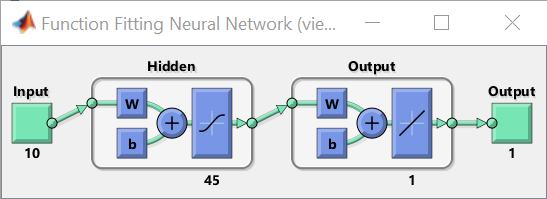
\includegraphics{img/arousal_mlp_45.png} 
	\caption{MLP Structure for arousal}
\end{figure}
\begin{figure}[H]
	\centering
	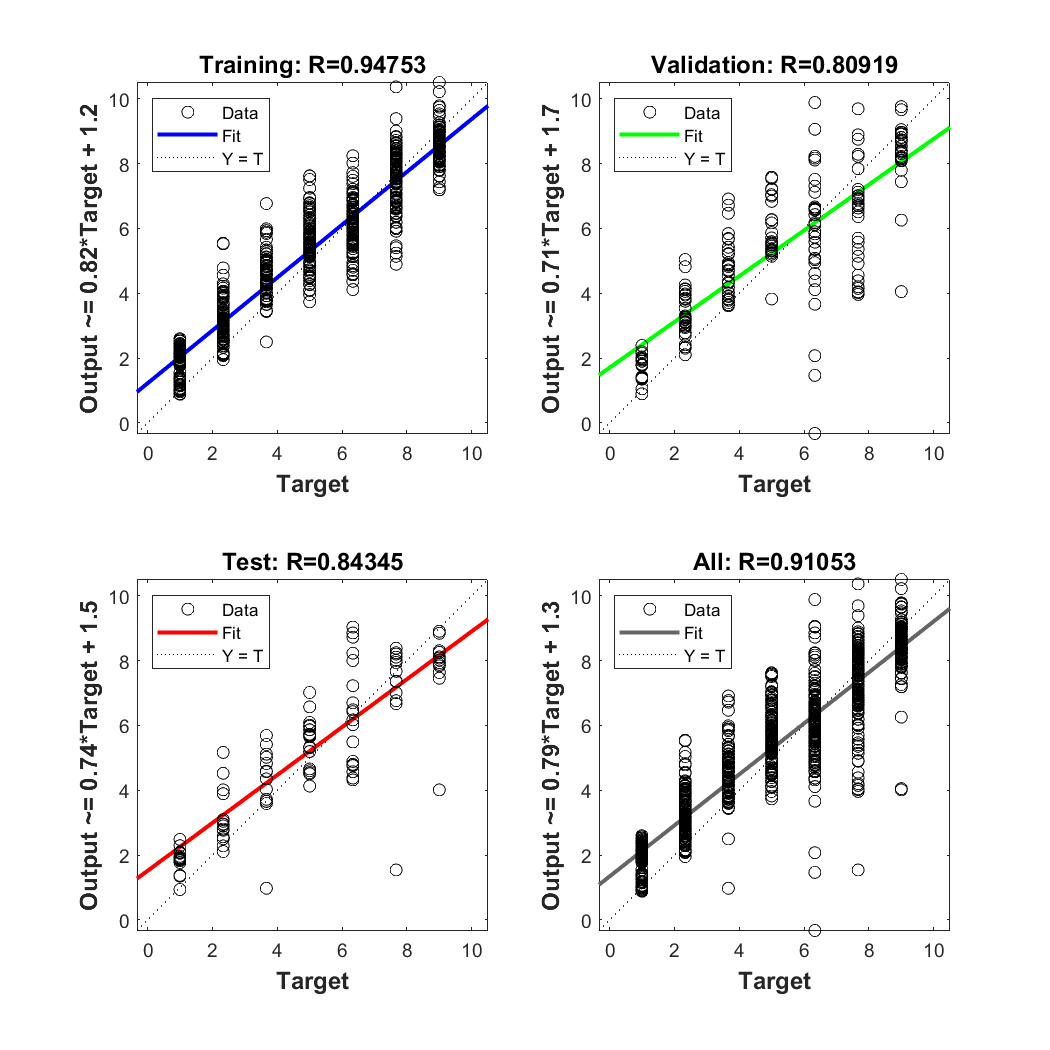
\includegraphics[width=\linewidth]{img/arousal_mlp_45_regression.png} 
	\caption{MLP Structure for arousal}
\end{figure}
\begin{figure}[H]
	\centering
	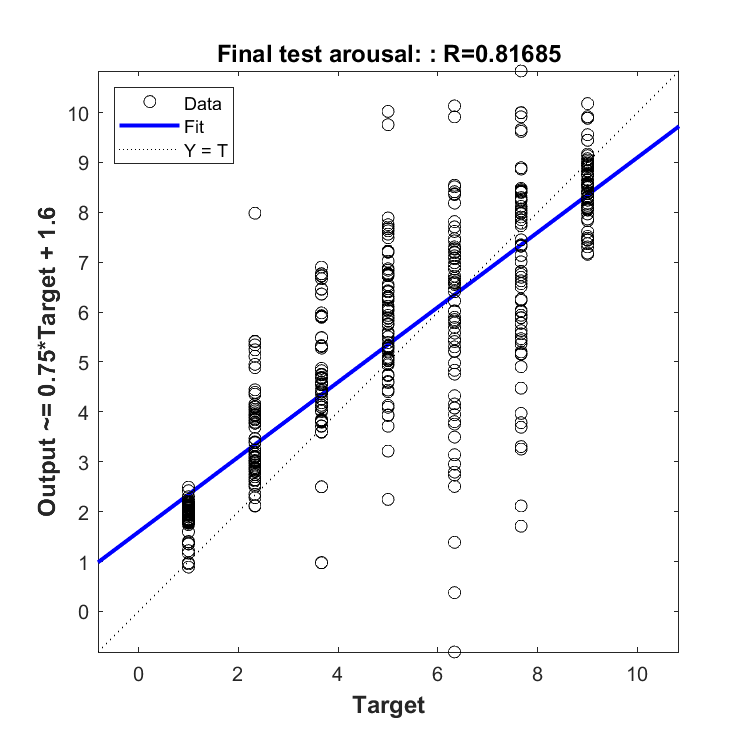
\includegraphics[width=0.6\linewidth]{img/arousal_mlp_45_regression_with_testset.png} 
	\caption{MLP Structure for arousal}
\end{figure}
\begin{figure}[H]
	\centering
	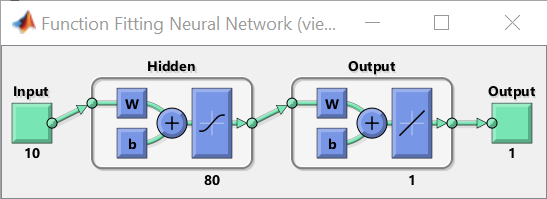
\includegraphics{img/valence_mlp_80.png} 
	\caption{MLP Structure for valence}
\end{figure}

\begin{figure}[H]
	\centering
	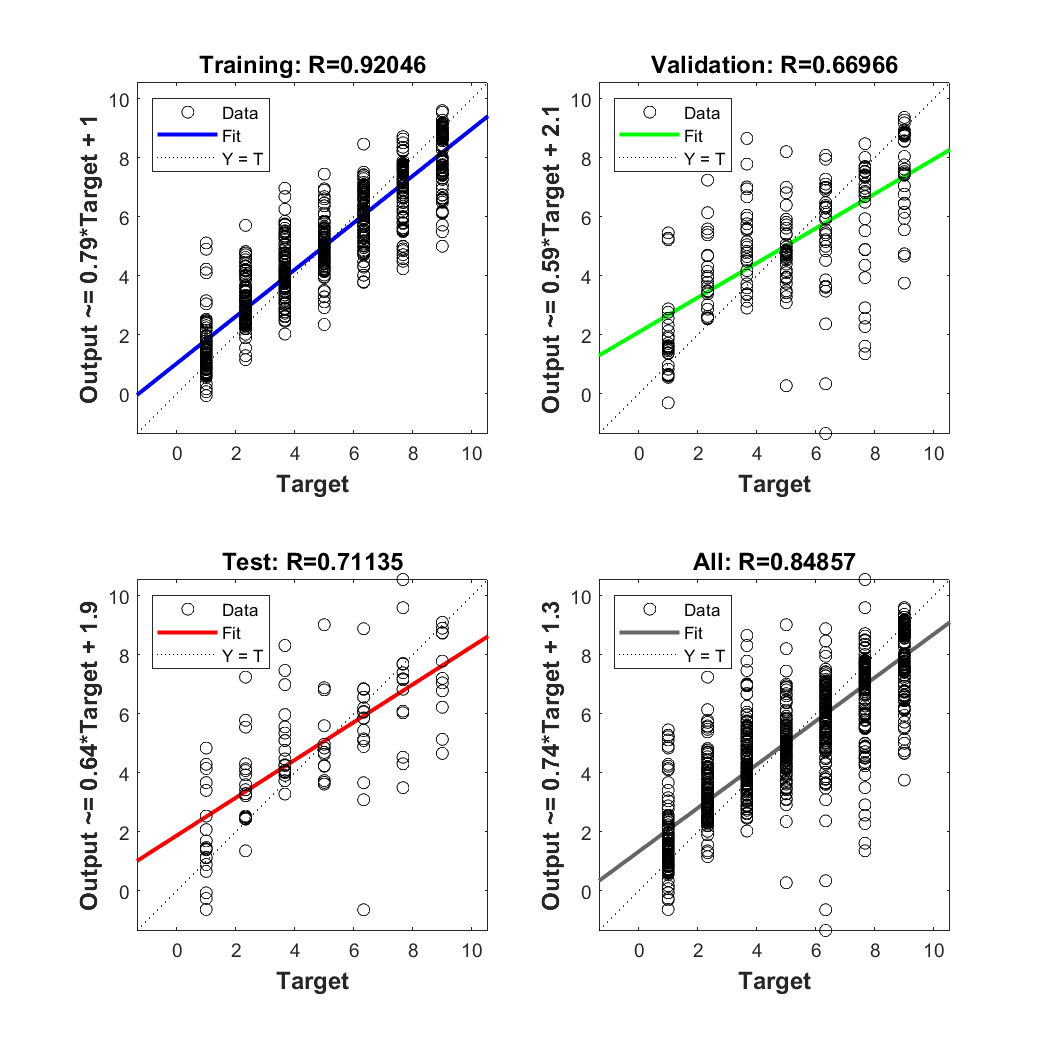
\includegraphics[width=\linewidth]{img/valence_mlp_80_regression.png} 
	\caption{Regression of MLP with Test Set}
\end{figure}
\begin{figure}[H]
	\centering
	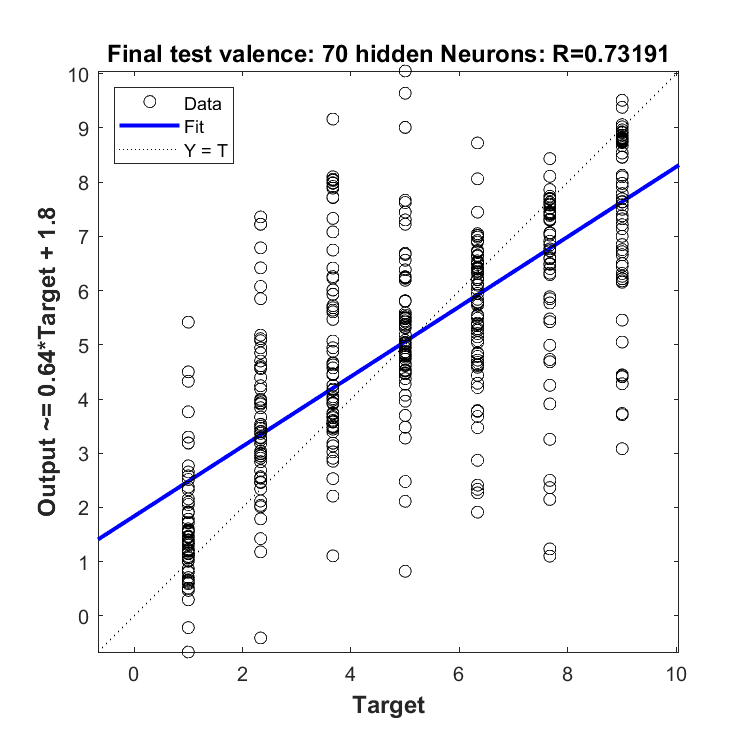
\includegraphics[width=0.6\linewidth]{img/valence_mlp_80_regression_with_testset.png} 
	\caption{Regression of MLP with Test Set}
\end{figure}

\subsection{RBF Training}
\begin{figure}[H]
	\centering
	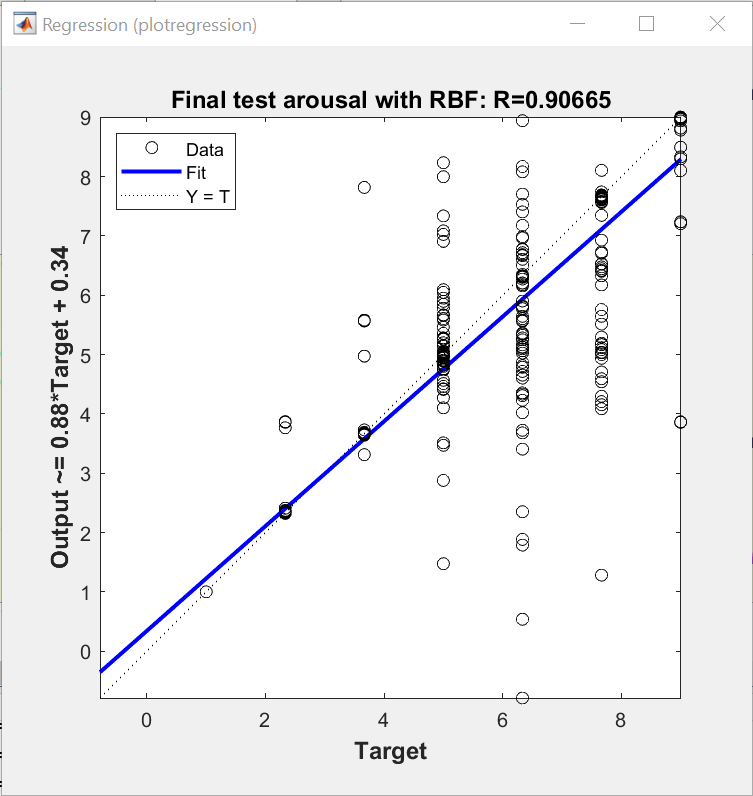
\includegraphics[width=0.6\linewidth]{img/arousal_rbf_1_3.png}
	\caption{Regression of MLP with Test Set}
\end{figure}
\begin{figure}[H]
	\centering
	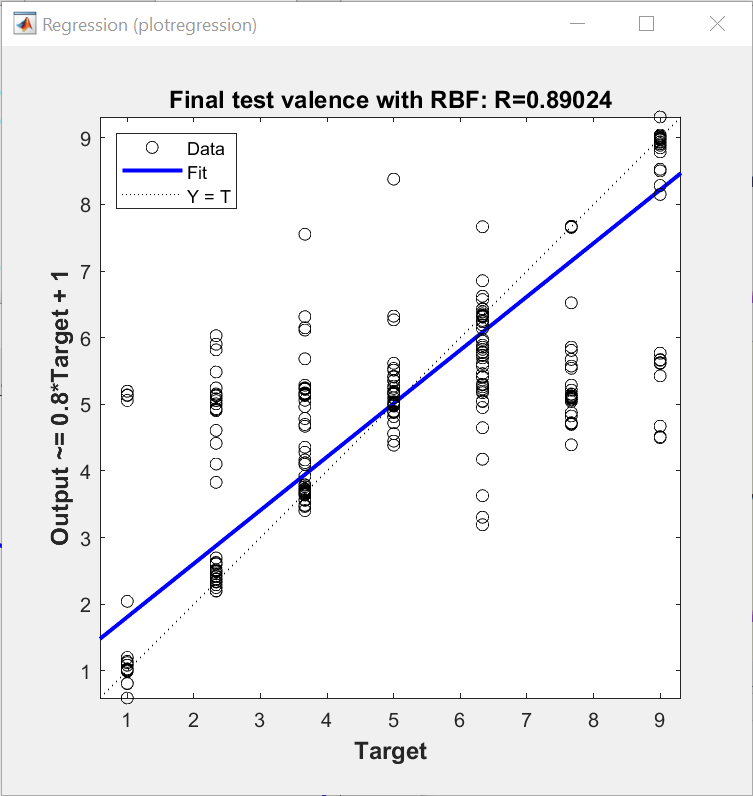
\includegraphics[width=0.6\linewidth]{img/valence_rbf_0_7.png}
	\caption{Regression of MLP with Test Set}
\end{figure}
